\documentclass[1p]{elsarticle_modified}
%\bibliographystyle{elsarticle-num}

%\usepackage[colorlinks]{hyperref}
%\usepackage{abbrmath_seonhwa} %\Abb, \Ascr, \Acal ,\Abf, \Afrak
\usepackage{amsfonts}
\usepackage{amssymb}
\usepackage{amsmath}
\usepackage{amsthm}
\usepackage{scalefnt}
\usepackage{amsbsy}
\usepackage{kotex}
\usepackage{caption}
\usepackage{subfig}
\usepackage{color}
\usepackage{graphicx}
\usepackage{xcolor} %% white, black, red, green, blue, cyan, magenta, yellow
\usepackage{float}
\usepackage{setspace}
\usepackage{hyperref}

\usepackage{tikz}
\usetikzlibrary{arrows}

\usepackage{multirow}
\usepackage{array} % fixed length table
\usepackage{hhline}

%%%%%%%%%%%%%%%%%%%%%
\makeatletter
\renewcommand*\env@matrix[1][\arraystretch]{%
	\edef\arraystretch{#1}%
	\hskip -\arraycolsep
	\let\@ifnextchar\new@ifnextchar
	\array{*\c@MaxMatrixCols c}}
\makeatother %https://tex.stackexchange.com/questions/14071/how-can-i-increase-the-line-spacing-in-a-matrix
%%%%%%%%%%%%%%%

\usepackage[normalem]{ulem}

\newcommand{\msout}[1]{\ifmmode\text{\sout{\ensuremath{#1}}}\else\sout{#1}\fi}
%SOURCE: \msout is \stkout macro in https://tex.stackexchange.com/questions/20609/strikeout-in-math-mode

\newcommand{\cancel}[1]{
	\ifmmode
	{\color{red}\msout{#1}}
	\else
	{\color{red}\sout{#1}}
	\fi
}

\newcommand{\add}[1]{
	{\color{blue}\uwave{#1}}
}

\newcommand{\replace}[2]{
	\ifmmode
	{\color{red}\msout{#1}}{\color{blue}\uwave{#2}}
	\else
	{\color{red}\sout{#1}}{\color{blue}\uwave{#2}}
	\fi
}

\newcommand{\Sol}{\mathcal{S}} %segment
\newcommand{\D}{D} %diagram
\newcommand{\A}{\mathcal{A}} %arc


%%%%%%%%%%%%%%%%%%%%%%%%%%%%%5 test

\def\sl{\operatorname{\textup{SL}}(2,\Cbb)}
\def\psl{\operatorname{\textup{PSL}}(2,\Cbb)}
\def\quan{\mkern 1mu \triangleright \mkern 1mu}

\theoremstyle{definition}
\newtheorem{thm}{Theorem}[section]
\newtheorem{prop}[thm]{Proposition}
\newtheorem{lem}[thm]{Lemma}
\newtheorem{ques}[thm]{Question}
\newtheorem{cor}[thm]{Corollary}
\newtheorem{defn}[thm]{Definition}
\newtheorem{exam}[thm]{Example}
\newtheorem{rmk}[thm]{Remark}
\newtheorem{alg}[thm]{Algorithm}

\newcommand{\I}{\sqrt{-1}}
\begin{document}

%\begin{frontmatter}
%
%\title{Boundary parabolic representations of knots up to 8 crossings}
%
%%% Group authors per affiliation:
%\author{Yunhi Cho} 
%\address{Department of Mathematics, University of Seoul, Seoul, Korea}
%\ead{yhcho@uos.ac.kr}
%
%
%\author{Seonhwa Kim} %\fnref{s_kim}}
%\address{Center for Geometry and Physics, Institute for Basic Science, Pohang, 37673, Korea}
%\ead{ryeona17@ibs.re.kr}
%
%\author{Hyuk Kim}
%\address{Department of Mathematical Sciences, Seoul National University, Seoul 08826, Korea}
%\ead{hyukkim@snu.ac.kr}
%
%\author{Seokbeom Yoon}
%\address{Department of Mathematical Sciences, Seoul National University, Seoul, 08826,  Korea}
%\ead{sbyoon15@snu.ac.kr}
%
%\begin{abstract}
%We find all boundary parabolic representation of knots up to 8 crossings.
%
%\end{abstract}
%\begin{keyword}
%    \MSC[2010] 57M25 
%\end{keyword}
%
%\end{frontmatter}

%\linenumbers
%\tableofcontents
%
\newcommand\colored[1]{\textcolor{white}{\rule[-0.35ex]{0.8em}{1.4ex}}\kern-0.8em\color{red} #1}%
%\newcommand\colored[1]{\textcolor{white}{ #1}\kern-2.17ex	\textcolor{white}{ #1}\kern-1.81ex	\textcolor{white}{ #1}\kern-2.15ex\color{red}#1	}

{\Large $\underline{12n_{0307}~(K12n_{0307})}$}

\setlength{\tabcolsep}{10pt}
\renewcommand{\arraystretch}{1.6}
\vspace{1cm}\begin{tabular}{m{100pt}>{\centering\arraybackslash}m{274pt}}
\multirow{5}{120pt}{
	\centering
	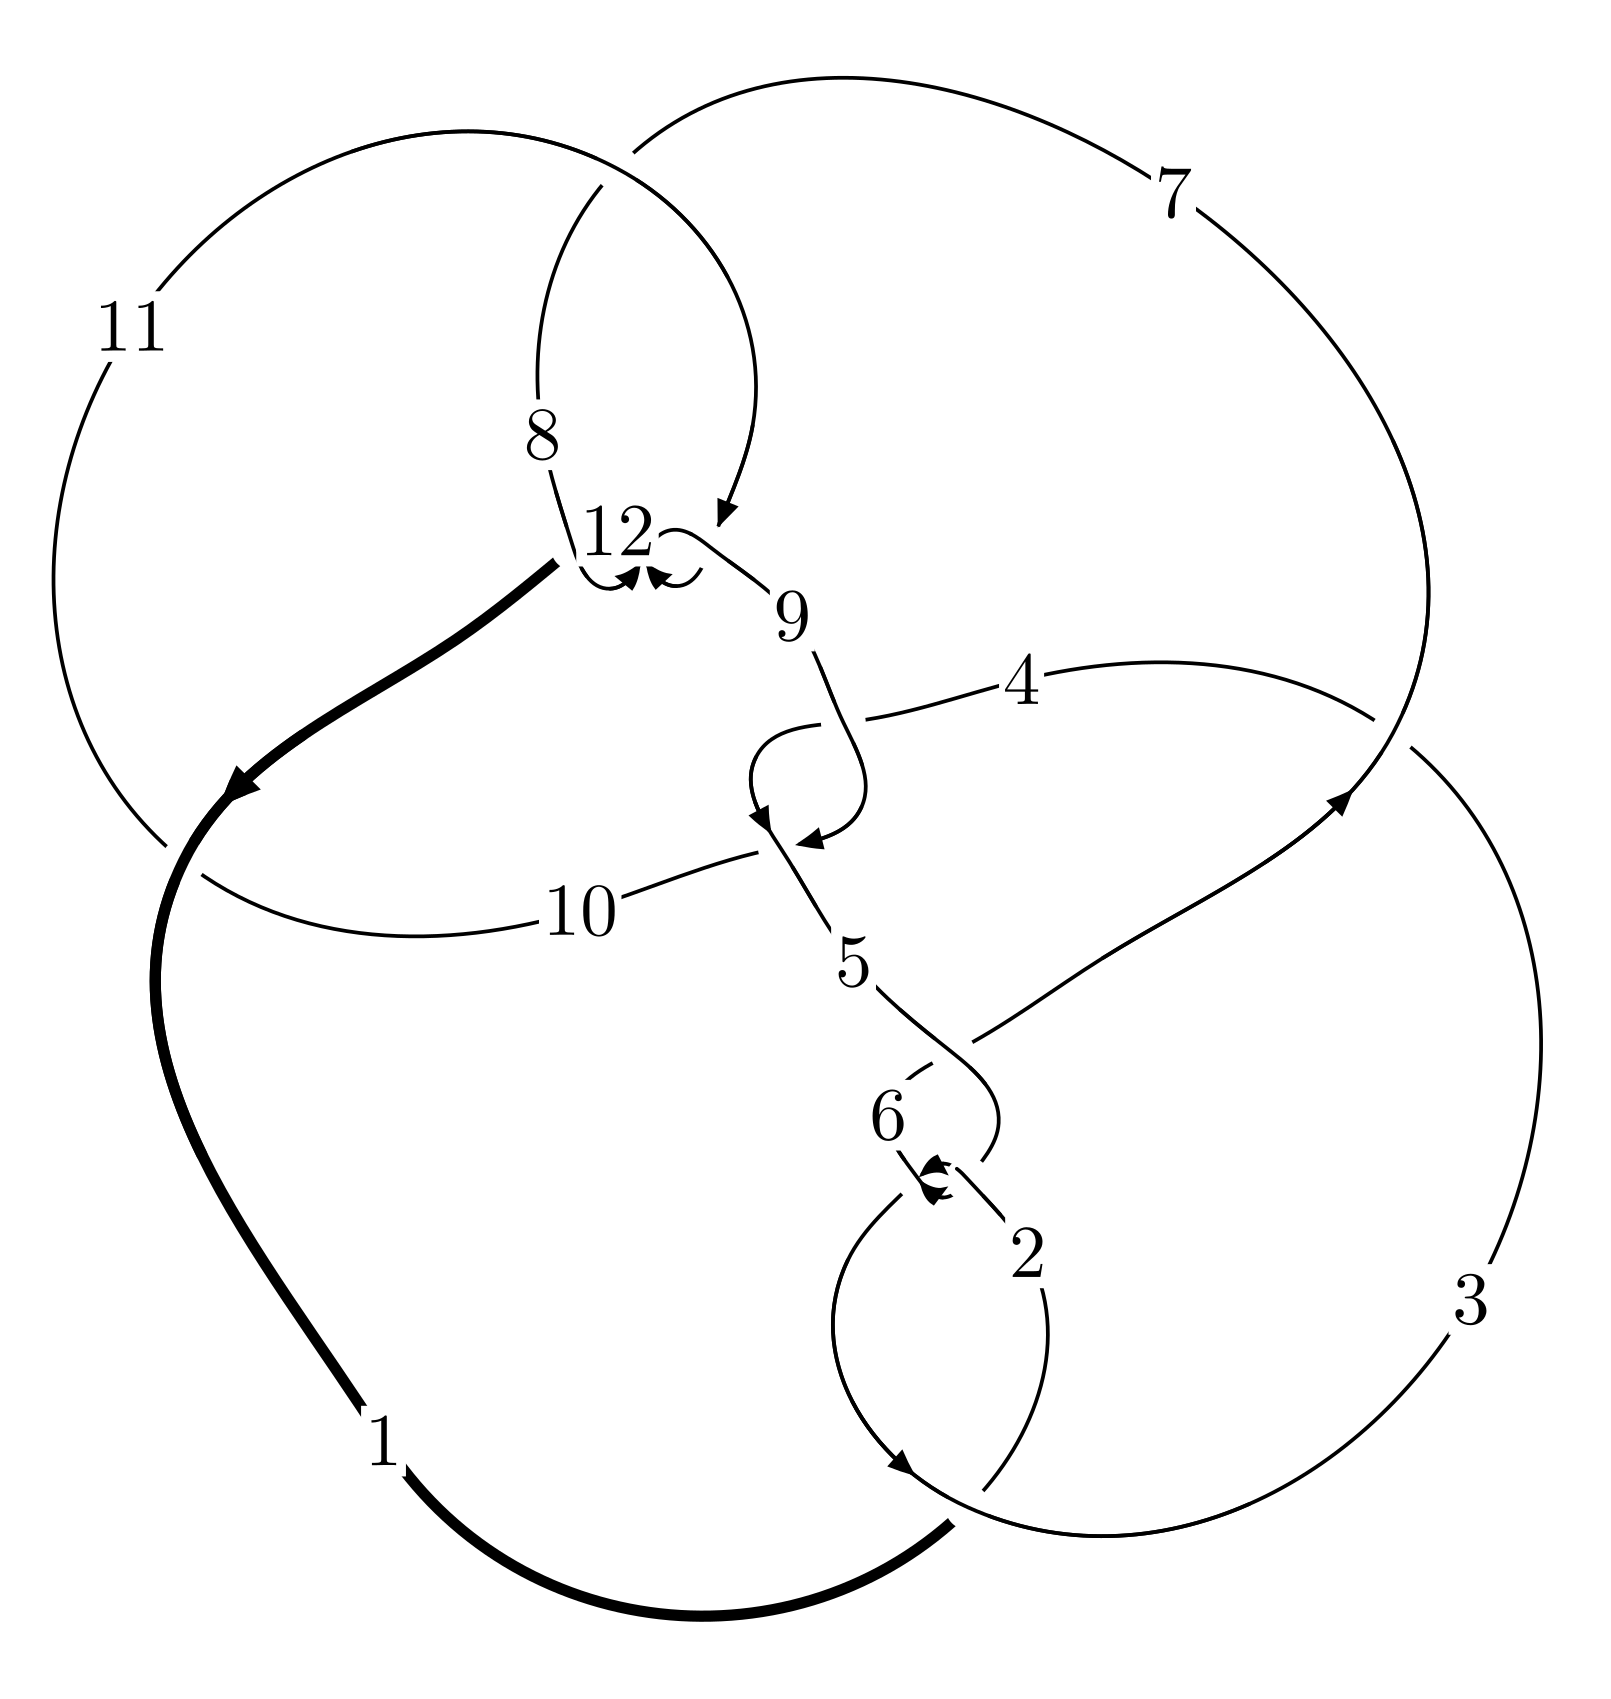
\includegraphics[width=112pt]{../../../GIT/diagram.site/Diagrams/png/2396_12n_0307.png}\\
\ \ \ A knot diagram\footnotemark}&
\allowdisplaybreaks
\textbf{Linearized knot diagam} \\
\cline{2-2}
 &
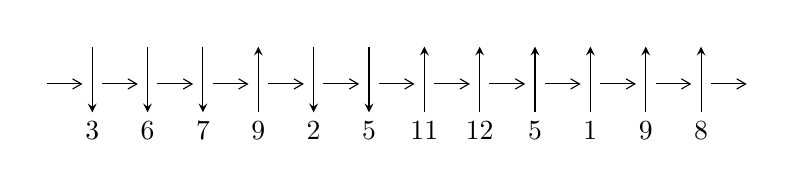
\begin{tikzpicture}[x=20pt, y=17pt]
	% nodes
	\node (C0) at (0, 0) {};
	\node (C1) at (1, 0) {};
	\node (C1U) at (1, +1) {};
	\node (C1D) at (1, -1) {3};

	\node (C2) at (2, 0) {};
	\node (C2U) at (2, +1) {};
	\node (C2D) at (2, -1) {6};

	\node (C3) at (3, 0) {};
	\node (C3U) at (3, +1) {};
	\node (C3D) at (3, -1) {7};

	\node (C4) at (4, 0) {};
	\node (C4U) at (4, +1) {};
	\node (C4D) at (4, -1) {9};

	\node (C5) at (5, 0) {};
	\node (C5U) at (5, +1) {};
	\node (C5D) at (5, -1) {2};

	\node (C6) at (6, 0) {};
	\node (C6U) at (6, +1) {};
	\node (C6D) at (6, -1) {5};

	\node (C7) at (7, 0) {};
	\node (C7U) at (7, +1) {};
	\node (C7D) at (7, -1) {11};

	\node (C8) at (8, 0) {};
	\node (C8U) at (8, +1) {};
	\node (C8D) at (8, -1) {12};

	\node (C9) at (9, 0) {};
	\node (C9U) at (9, +1) {};
	\node (C9D) at (9, -1) {5};

	\node (C10) at (10, 0) {};
	\node (C10U) at (10, +1) {};
	\node (C10D) at (10, -1) {1};

	\node (C11) at (11, 0) {};
	\node (C11U) at (11, +1) {};
	\node (C11D) at (11, -1) {9};

	\node (C12) at (12, 0) {};
	\node (C12U) at (12, +1) {};
	\node (C12D) at (12, -1) {8};
	\node (C13) at (13, 0) {};

	% arrows
	\draw[->,>={angle 60}]
	(C0) edge (C1) (C1) edge (C2) (C2) edge (C3) (C3) edge (C4) (C4) edge (C5) (C5) edge (C6) (C6) edge (C7) (C7) edge (C8) (C8) edge (C9) (C9) edge (C10) (C10) edge (C11) (C11) edge (C12) (C12) edge (C13) ;	\draw[->,>=stealth]
	(C1U) edge (C1D) (C2U) edge (C2D) (C3U) edge (C3D) (C4D) edge (C4U) (C5U) edge (C5D) (C6U) edge (C6D) (C7D) edge (C7U) (C8D) edge (C8U) (C9D) edge (C9U) (C10D) edge (C10U) (C11D) edge (C11U) (C12D) edge (C12U) ;
	\end{tikzpicture} \\
\hhline{~~} \\& 
\textbf{Solving Sequence} \\ \cline{2-2} 
 &
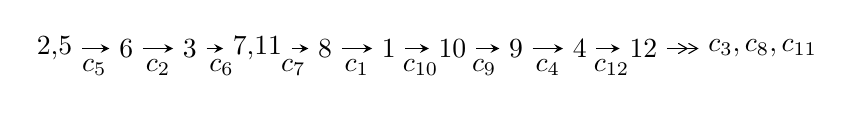
\begin{tikzpicture}[x=23pt, y=7pt]
	% node
	\node (A0) at (-1/8, 0) {2,5};
	\node (A1) at (1, 0) {6};
	\node (A2) at (2, 0) {3};
	\node (A3) at (49/16, 0) {7,11};
	\node (A4) at (33/8, 0) {8};
	\node (A5) at (41/8, 0) {1};
	\node (A6) at (49/8, 0) {10};
	\node (A7) at (57/8, 0) {9};
	\node (A8) at (65/8, 0) {4};
	\node (A9) at (73/8, 0) {12};
	\node (C1) at (1/2, -1) {$c_{5}$};
	\node (C2) at (3/2, -1) {$c_{2}$};
	\node (C3) at (5/2, -1) {$c_{6}$};
	\node (C4) at (29/8, -1) {$c_{7}$};
	\node (C5) at (37/8, -1) {$c_{1}$};
	\node (C6) at (45/8, -1) {$c_{10}$};
	\node (C7) at (53/8, -1) {$c_{9}$};
	\node (C8) at (61/8, -1) {$c_{4}$};
	\node (C9) at (69/8, -1) {$c_{12}$};
	\node (A10) at (11, 0) {$c_{3},c_{8},c_{11}$};

	% edge
	\draw[->,>=stealth]	
	(A0) edge (A1) (A1) edge (A2) (A2) edge (A3) (A3) edge (A4) (A4) edge (A5) (A5) edge (A6) (A6) edge (A7) (A7) edge (A8) (A8) edge (A9) ;
	\draw[->>,>={angle 60}]	
	(A9) edge (A10);
\end{tikzpicture} \\ 

\end{tabular} \\

\footnotetext{
The image of knot diagram is generated by the software ``\textbf{Draw programme}" developed by Andrew Bartholomew(\url{http://www.layer8.co.uk/maths/draw/index.htm\#Running-draw}), where we modified some parts for our purpose(\url{https://github.com/CATsTAILs/LinksPainter}).
}\phantom \\ \newline 
\centering \textbf{Ideals for irreducible components\footnotemark of $X_{\text{par}}$} 
 
\begin{align*}
I^u_{1}&=\langle 
-28 u^{46}-99 u^{45}+\cdots+4 b+28,\;-8 u^{46}-13 u^{45}+\cdots+4 a+9,\;u^{47}+4 u^{46}+\cdots+3 u-1\rangle \\
I^u_{2}&=\langle 
- u^2 a+b+a,\;u^2 a+a^2- a u+u^2+a- u+1,\;u^3- u^2+1\rangle \\
I^u_{3}&=\langle 
- u^2+b+1,\;a-1,\;u^3- u^2+1\rangle \\
\\
\end{align*}
\raggedright * 3 irreducible components of $\dim_{\mathbb{C}}=0$, with total 56 representations.\\
\footnotetext{All coefficients of polynomials are rational numbers. But the coefficients are sometimes approximated in decimal forms when there is not enough margin.}
\newpage
\renewcommand{\arraystretch}{1}
\centering \section*{I. $I^u_{1}= \langle -28 u^{46}-99 u^{45}+\cdots+4 b+28,\;-8 u^{46}-13 u^{45}+\cdots+4 a+9,\;u^{47}+4 u^{46}+\cdots+3 u-1 \rangle$}
\flushleft \textbf{(i) Arc colorings}\\
\begin{tabular}{m{7pt} m{180pt} m{7pt} m{180pt} }
\flushright $a_{2}=$&$\begin{pmatrix}0\\u\end{pmatrix}$ \\
\flushright $a_{5}=$&$\begin{pmatrix}1\\0\end{pmatrix}$ \\
\flushright $a_{6}=$&$\begin{pmatrix}1\\u^2\end{pmatrix}$ \\
\flushright $a_{3}=$&$\begin{pmatrix}- u\\- u^3+u\end{pmatrix}$ \\
\flushright $a_{7}=$&$\begin{pmatrix}- u^2+1\\u^2\end{pmatrix}$ \\
\flushright $a_{11}=$&$\begin{pmatrix}2 u^{46}+\frac{13}{4} u^{45}+\cdots-\frac{11}{2} u-\frac{9}{4}\\7 u^{46}+\frac{99}{4} u^{45}+\cdots+\frac{113}{4} u-7\end{pmatrix}$ \\
\flushright $a_{8}=$&$\begin{pmatrix}\frac{1}{4} u^{45}+\frac{3}{4} u^{44}+\cdots+\frac{13}{4} u+2\\-\frac{1}{4} u^{46}- u^{45}+\cdots-2 u+\frac{1}{4}\end{pmatrix}$ \\
\flushright $a_{1}=$&$\begin{pmatrix}u^3\\u^5- u^3+u\end{pmatrix}$ \\
\flushright $a_{10}=$&$\begin{pmatrix}\frac{23}{4} u^{46}+\frac{39}{2} u^{45}+\cdots+\frac{41}{2} u-\frac{35}{4}\\\frac{7}{2} u^{46}+12 u^{45}+\cdots+15 u-\frac{7}{2}\end{pmatrix}$ \\
\flushright $a_{9}=$&$\begin{pmatrix}\frac{9}{4} u^{46}+\frac{15}{2} u^{45}+\cdots+\frac{11}{2} u-\frac{21}{4}\\\frac{7}{2} u^{46}+12 u^{45}+\cdots+15 u-\frac{7}{2}\end{pmatrix}$ \\
\flushright $a_{4}=$&$\begin{pmatrix}u^7-2 u^5+2 u^3-2 u\\- u^7+u^5-2 u^3+u\end{pmatrix}$ \\
\flushright $a_{12}=$&$\begin{pmatrix}-\frac{7}{4} u^{45}-\frac{19}{4} u^{44}+\cdots-\frac{31}{4} u+\frac{1}{2}\\3 u^{46}+\frac{43}{4} u^{45}+\cdots+\frac{49}{4} u-3\end{pmatrix}$\\&\end{tabular}
\flushleft \textbf{(ii) Obstruction class $= -1$}\\~\\
\flushleft \textbf{(iii) Cusp Shapes $= \frac{67}{4} u^{46}+\frac{101}{2} u^{45}+\cdots+\frac{225}{4} u-\frac{3}{2}$}\\~\\
\newpage\renewcommand{\arraystretch}{1}
\flushleft \textbf{(iv) u-Polynomials at the component}\newline \\
\begin{tabular}{m{50pt}|m{274pt}}
Crossings & \hspace{64pt}u-Polynomials at each crossing \\
\hline $$\begin{aligned}c_{1},c_{6}\end{aligned}$$&$\begin{aligned}
&u^{47}+18 u^{46}+\cdots+35 u+1
\end{aligned}$\\
\hline $$\begin{aligned}c_{2},c_{5}\end{aligned}$$&$\begin{aligned}
&u^{47}+4 u^{46}+\cdots+3 u-1
\end{aligned}$\\
\hline $$\begin{aligned}c_{3}\end{aligned}$$&$\begin{aligned}
&u^{47}-4 u^{46}+\cdots+9 u-1
\end{aligned}$\\
\hline $$\begin{aligned}c_{4},c_{9}\end{aligned}$$&$\begin{aligned}
&u^{47}- u^{46}+\cdots-1024 u-512
\end{aligned}$\\
\hline $$\begin{aligned}c_{7}\end{aligned}$$&$\begin{aligned}
&u^{47}-4 u^{46}+\cdots-4441 u-1153
\end{aligned}$\\
\hline $$\begin{aligned}c_{8},c_{11},c_{12}\end{aligned}$$&$\begin{aligned}
&u^{47}+4 u^{46}+\cdots-5 u-1
\end{aligned}$\\
\hline $$\begin{aligned}c_{10}\end{aligned}$$&$\begin{aligned}
&u^{47}+6 u^{46}+\cdots-31 u-3
\end{aligned}$\\
\hline
\end{tabular}\\~\\
\newpage\renewcommand{\arraystretch}{1}
\flushleft \textbf{(v) Riley Polynomials at the component}\newline \\
\begin{tabular}{m{50pt}|m{274pt}}
Crossings & \hspace{64pt}Riley Polynomials at each crossing \\
\hline $$\begin{aligned}c_{1},c_{6}\end{aligned}$$&$\begin{aligned}
&y^{47}+26 y^{46}+\cdots+787 y-1
\end{aligned}$\\
\hline $$\begin{aligned}c_{2},c_{5}\end{aligned}$$&$\begin{aligned}
&y^{47}-18 y^{46}+\cdots+35 y-1
\end{aligned}$\\
\hline $$\begin{aligned}c_{3}\end{aligned}$$&$\begin{aligned}
&y^{47}-58 y^{46}+\cdots+35 y-1
\end{aligned}$\\
\hline $$\begin{aligned}c_{4},c_{9}\end{aligned}$$&$\begin{aligned}
&y^{47}+49 y^{46}+\cdots-1703936 y-262144
\end{aligned}$\\
\hline $$\begin{aligned}c_{7}\end{aligned}$$&$\begin{aligned}
&y^{47}+22 y^{46}+\cdots-27059341 y-1329409
\end{aligned}$\\
\hline $$\begin{aligned}c_{8},c_{11},c_{12}\end{aligned}$$&$\begin{aligned}
&y^{47}+46 y^{46}+\cdots-5 y-1
\end{aligned}$\\
\hline $$\begin{aligned}c_{10}\end{aligned}$$&$\begin{aligned}
&y^{47}+50 y^{46}+\cdots+475 y-9
\end{aligned}$\\
\hline
\end{tabular}\\~\\
\newpage\flushleft \textbf{(vi) Complex Volumes and Cusp Shapes}
$$\begin{array}{c|c|c}  
\text{Solutions to }I^u_{1}& \I (\text{vol} + \sqrt{-1}CS) & \text{Cusp shape}\\
 \hline 
\begin{aligned}
u &= -0.542579 + 0.845522 I \\
a &= \phantom{-}0.52046 - 1.65523 I \\
b &= -0.81563 + 1.38652 I\end{aligned}
 & -2.89318 - 4.02038 I & \phantom{-}2.80109 + 3.23953 I \\ \hline\begin{aligned}
u &= -0.542579 - 0.845522 I \\
a &= \phantom{-}0.52046 + 1.65523 I \\
b &= -0.81563 - 1.38652 I\end{aligned}
 & -2.89318 + 4.02038 I & \phantom{-}2.80109 - 3.23953 I \\ \hline\begin{aligned}
u &= -0.849325 + 0.570079 I \\
a &= \phantom{-}0.646245 + 0.025782 I \\
b &= \phantom{-}0.284968 - 1.290140 I\end{aligned}
 & \phantom{-}2.17863 + 2.27566 I & \phantom{-}3.19435 - 3.09284 I \\ \hline\begin{aligned}
u &= -0.849325 - 0.570079 I \\
a &= \phantom{-}0.646245 - 0.025782 I \\
b &= \phantom{-}0.284968 + 1.290140 I\end{aligned}
 & \phantom{-}2.17863 - 2.27566 I & \phantom{-}3.19435 + 3.09284 I \\ \hline\begin{aligned}
u &= -0.406871 + 0.865991 I \\
a &= -0.021631 - 1.238880 I \\
b &= \phantom{-}0.731358 + 1.204980 I\end{aligned}
 & -9.98450 + 3.38049 I & -1.32078 - 2.56603 I \\ \hline\begin{aligned}
u &= -0.406871 - 0.865991 I \\
a &= -0.021631 + 1.238880 I \\
b &= \phantom{-}0.731358 - 1.204980 I\end{aligned}
 & -9.98450 - 3.38049 I & -1.32078 + 2.56603 I \\ \hline\begin{aligned}
u &= -0.750352 + 0.593025 I \\
a &= -1.020220 + 0.373354 I \\
b &= \phantom{-}0.367043 + 1.185280 I\end{aligned}
 & -1.34099 - 1.39615 I & -0.069604 + 1.411136 I \\ \hline\begin{aligned}
u &= -0.750352 - 0.593025 I \\
a &= -1.020220 - 0.373354 I \\
b &= \phantom{-}0.367043 - 1.185280 I\end{aligned}
 & -1.34099 + 1.39615 I & -0.069604 - 1.411136 I \\ \hline\begin{aligned}
u &= -0.559716 + 0.892329 I \\
a &= -0.45129 + 1.94560 I \\
b &= \phantom{-}1.07277 - 2.03235 I\end{aligned}
 & -9.05378 - 7.60668 I & -0.58639 + 3.22129 I \\ \hline\begin{aligned}
u &= -0.559716 - 0.892329 I \\
a &= -0.45129 - 1.94560 I \\
b &= \phantom{-}1.07277 + 2.03235 I\end{aligned}
 & -9.05378 + 7.60668 I & -0.58639 - 3.22129 I\\
 \hline 
 \end{array}$$\newpage$$\begin{array}{c|c|c}  
\text{Solutions to }I^u_{1}& \I (\text{vol} + \sqrt{-1}CS) & \text{Cusp shape}\\
 \hline 
\begin{aligned}
u &= -1.035120 + 0.209994 I \\
a &= \phantom{-}0.882211 - 0.713191 I \\
b &= \phantom{-}0.774400 - 0.897748 I\end{aligned}
 & -6.95929 - 0.03774 I & -5.96271 - 0.75839 I \\ \hline\begin{aligned}
u &= -1.035120 - 0.209994 I \\
a &= \phantom{-}0.882211 + 0.713191 I \\
b &= \phantom{-}0.774400 + 0.897748 I\end{aligned}
 & -6.95929 + 0.03774 I & -5.96271 + 0.75839 I \\ \hline\begin{aligned}
u &= \phantom{-}0.766231 + 0.547591 I \\
a &= -1.65889 - 0.74494 I \\
b &= \phantom{-}1.179640 - 0.111554 I\end{aligned}
 & \phantom{-}1.49256 - 0.66743 I & \phantom{-}4.54233 - 0.09202 I \\ \hline\begin{aligned}
u &= \phantom{-}0.766231 - 0.547591 I \\
a &= -1.65889 + 0.74494 I \\
b &= \phantom{-}1.179640 + 0.111554 I\end{aligned}
 & \phantom{-}1.49256 + 0.66743 I & \phantom{-}4.54233 + 0.09202 I \\ \hline\begin{aligned}
u &= -0.472512 + 0.810458 I \\
a &= -0.352292 + 1.319250 I \\
b &= \phantom{-}0.091933 - 0.956029 I\end{aligned}
 & -3.35426 + 0.41641 I & \phantom{-}1.81917 - 2.68288 I \\ \hline\begin{aligned}
u &= -0.472512 - 0.810458 I \\
a &= -0.352292 - 1.319250 I \\
b &= \phantom{-}0.091933 + 0.956029 I\end{aligned}
 & -3.35426 - 0.41641 I & \phantom{-}1.81917 + 2.68288 I \\ \hline\begin{aligned}
u &= \phantom{-}0.916719 + 0.584389 I \\
a &= \phantom{-}1.43793 + 1.12449 I \\
b &= -1.185440 + 0.406825 I\end{aligned}
 & \phantom{-}0.99495 - 3.89558 I & \phantom{-}2.00000 + 7.22930 I \\ \hline\begin{aligned}
u &= \phantom{-}0.916719 - 0.584389 I \\
a &= \phantom{-}1.43793 - 1.12449 I \\
b &= -1.185440 - 0.406825 I\end{aligned}
 & \phantom{-}0.99495 + 3.89558 I & \phantom{-}2.00000 - 7.22930 I \\ \hline\begin{aligned}
u &= -0.919108 + 0.591025 I \\
a &= -0.158662 - 0.317671 I \\
b &= -0.820356 + 1.073340 I\end{aligned}
 & -1.86367 + 6.09961 I & -1.78165 - 6.44137 I \\ \hline\begin{aligned}
u &= -0.919108 - 0.591025 I \\
a &= -0.158662 + 0.317671 I \\
b &= -0.820356 - 1.073340 I\end{aligned}
 & -1.86367 - 6.09961 I & -1.78165 + 6.44137 I\\
 \hline 
 \end{array}$$\newpage$$\begin{array}{c|c|c}  
\text{Solutions to }I^u_{1}& \I (\text{vol} + \sqrt{-1}CS) & \text{Cusp shape}\\
 \hline 
\begin{aligned}
u &= \phantom{-}0.807896 + 0.791990 I \\
a &= \phantom{-}1.46759 - 0.27866 I \\
b &= -1.13467 + 1.37041 I\end{aligned}
 & -0.27990 - 1.40024 I & \phantom{-0.000000 -}0. + 3.69287 I \\ \hline\begin{aligned}
u &= \phantom{-}0.807896 - 0.791990 I \\
a &= \phantom{-}1.46759 + 0.27866 I \\
b &= -1.13467 - 1.37041 I\end{aligned}
 & -0.27990 + 1.40024 I & \phantom{-0.000000 } 0. - 3.69287 I \\ \hline\begin{aligned}
u &= \phantom{-}1.005160 + 0.543180 I \\
a &= -1.74932 - 1.37109 I \\
b &= \phantom{-}1.071900 - 0.860916 I\end{aligned}
 & -5.01656 - 6.25958 I & -2.44147 + 6.00005 I \\ \hline\begin{aligned}
u &= \phantom{-}1.005160 - 0.543180 I \\
a &= -1.74932 + 1.37109 I \\
b &= \phantom{-}1.071900 + 0.860916 I\end{aligned}
 & -5.01656 + 6.25958 I & -2.44147 - 6.00005 I \\ \hline\begin{aligned}
u &= \phantom{-}0.880391 + 0.769089 I \\
a &= -0.562518 + 0.643186 I \\
b &= -0.135747 - 0.962284 I\end{aligned}
 & \phantom{-}3.63076 - 2.90147 I & -4.60953 + 3.97403 I \\ \hline\begin{aligned}
u &= \phantom{-}0.880391 - 0.769089 I \\
a &= -0.562518 - 0.643186 I \\
b &= -0.135747 + 0.962284 I\end{aligned}
 & \phantom{-}3.63076 + 2.90147 I & -4.60953 - 3.97403 I \\ \hline\begin{aligned}
u &= \phantom{-}1.175580 + 0.026203 I \\
a &= \phantom{-}0.226154 - 0.429398 I \\
b &= \phantom{-}0.18576 - 1.60517 I\end{aligned}
 & -9.13930 - 2.39543 I & -3.30646 + 2.93927 I \\ \hline\begin{aligned}
u &= \phantom{-}1.175580 - 0.026203 I \\
a &= \phantom{-}0.226154 + 0.429398 I \\
b &= \phantom{-}0.18576 + 1.60517 I\end{aligned}
 & -9.13930 + 2.39543 I & -3.30646 - 2.93927 I \\ \hline\begin{aligned}
u &= -0.797096 + 0.147471 I \\
a &= -0.470761 + 0.404647 I \\
b &= -0.305079 + 0.399977 I\end{aligned}
 & -1.341120 + 0.348467 I & -5.61848 - 0.75974 I \\ \hline\begin{aligned}
u &= -0.797096 - 0.147471 I \\
a &= -0.470761 - 0.404647 I \\
b &= -0.305079 - 0.399977 I\end{aligned}
 & -1.341120 - 0.348467 I & -5.61848 + 0.75974 I\\
 \hline 
 \end{array}$$\newpage$$\begin{array}{c|c|c}  
\text{Solutions to }I^u_{1}& \I (\text{vol} + \sqrt{-1}CS) & \text{Cusp shape}\\
 \hline 
\begin{aligned}
u &= \phantom{-}0.710745 + 0.353826 I \\
a &= \phantom{-}1.99025 + 0.84733 I \\
b &= -0.945738 - 0.231377 I\end{aligned}
 & -3.72397 + 2.21391 I & \phantom{-}0.64719 + 2.18592 I \\ \hline\begin{aligned}
u &= \phantom{-}0.710745 - 0.353826 I \\
a &= \phantom{-}1.99025 - 0.84733 I \\
b &= -0.945738 + 0.231377 I\end{aligned}
 & -3.72397 - 2.21391 I & \phantom{-}0.64719 - 2.18592 I \\ \hline\begin{aligned}
u &= \phantom{-}1.210150 + 0.061384 I \\
a &= -0.556915 + 0.710918 I \\
b &= -0.53977 + 1.79323 I\end{aligned}
 & -15.7778 - 5.9089 I & -6.14260 + 0. I\phantom{ +0.000000I} \\ \hline\begin{aligned}
u &= \phantom{-}1.210150 - 0.061384 I \\
a &= -0.556915 - 0.710918 I \\
b &= -0.53977 - 1.79323 I\end{aligned}
 & -15.7778 + 5.9089 I & -6.14260 + 0. I\phantom{ +0.000000I} \\ \hline\begin{aligned}
u &= \phantom{-}0.941818 + 0.771815 I \\
a &= \phantom{-}0.18006 - 1.54737 I \\
b &= \phantom{-}1.40667 + 1.15010 I\end{aligned}
 & -0.67750 - 4.47945 I & \phantom{-0.000000 } 0 \\ \hline\begin{aligned}
u &= \phantom{-}0.941818 - 0.771815 I \\
a &= \phantom{-}0.18006 + 1.54737 I \\
b &= \phantom{-}1.40667 - 1.15010 I\end{aligned}
 & -0.67750 + 4.47945 I & \phantom{-0.000000 } 0 \\ \hline\begin{aligned}
u &= -1.083300 + 0.641319 I \\
a &= \phantom{-}1.62476 + 0.25908 I \\
b &= -0.486943 - 1.100850 I\end{aligned}
 & -5.15574 + 5.00343 I & \phantom{-0.000000 } 0 \\ \hline\begin{aligned}
u &= -1.083300 - 0.641319 I \\
a &= \phantom{-}1.62476 - 0.25908 I \\
b &= -0.486943 + 1.100850 I\end{aligned}
 & -5.15574 - 5.00343 I & \phantom{-0.000000 } 0 \\ \hline\begin{aligned}
u &= -1.082000 + 0.677407 I \\
a &= -2.00058 + 0.02197 I \\
b &= \phantom{-}0.94583 + 1.66881 I\end{aligned}
 & -4.51999 + 9.69823 I & \phantom{-0.000000 } 0 \\ \hline\begin{aligned}
u &= -1.082000 - 0.677407 I \\
a &= -2.00058 - 0.02197 I \\
b &= \phantom{-}0.94583 - 1.66881 I\end{aligned}
 & -4.51999 - 9.69823 I & \phantom{-0.000000 } 0\\
 \hline 
 \end{array}$$\newpage$$\begin{array}{c|c|c}  
\text{Solutions to }I^u_{1}& \I (\text{vol} + \sqrt{-1}CS) & \text{Cusp shape}\\
 \hline 
\begin{aligned}
u &= -1.122540 + 0.615470 I \\
a &= -1.60372 - 0.82721 I \\
b &= -0.358676 + 1.009600 I\end{aligned}
 & -12.16410 + 2.06990 I & \phantom{-0.000000 } 0 \\ \hline\begin{aligned}
u &= -1.122540 - 0.615470 I \\
a &= -1.60372 + 0.82721 I \\
b &= -0.358676 - 1.009600 I\end{aligned}
 & -12.16410 - 2.06990 I & \phantom{-0.000000 } 0 \\ \hline\begin{aligned}
u &= -1.095820 + 0.699570 I \\
a &= \phantom{-}2.36060 - 0.03371 I \\
b &= -1.00797 - 2.27284 I\end{aligned}
 & -10.6948 + 13.4951 I & \phantom{-0.000000 } 0 \\ \hline\begin{aligned}
u &= -1.095820 - 0.699570 I \\
a &= \phantom{-}2.36060 + 0.03371 I \\
b &= -1.00797 + 2.27284 I\end{aligned}
 & -10.6948 - 13.4951 I & \phantom{-0.000000 } 0 \\ \hline\begin{aligned}
u &= \phantom{-}0.207923 + 0.417127 I \\
a &= \phantom{-}1.69044 - 0.06549 I \\
b &= -0.631998 - 0.720191 I\end{aligned}
 & -3.46548 + 2.21318 I & \phantom{-}2.85688 - 2.29805 I \\ \hline\begin{aligned}
u &= \phantom{-}0.207923 - 0.417127 I \\
a &= \phantom{-}1.69044 + 0.06549 I \\
b &= -0.631998 + 0.720191 I\end{aligned}
 & -3.46548 - 2.21318 I & \phantom{-}2.85688 + 2.29805 I \\ \hline\begin{aligned}
u &= \phantom{-}0.187442\phantom{ +0.000000I} \\
a &= -2.83979\phantom{ +0.000000I} \\
b &= \phantom{-}0.511458\phantom{ +0.000000I}\end{aligned}
 & \phantom{-}0.826035\phantom{ +0.000000I} & \phantom{-}12.4720\phantom{ +0.000000I}\\
 \hline 
 \end{array}$$\newpage\newpage\renewcommand{\arraystretch}{1}
\centering \section*{II. $I^u_{2}= \langle - u^2 a+b+a,\;u^2 a+a^2- a u+u^2+a- u+1,\;u^3- u^2+1 \rangle$}
\flushleft \textbf{(i) Arc colorings}\\
\begin{tabular}{m{7pt} m{180pt} m{7pt} m{180pt} }
\flushright $a_{2}=$&$\begin{pmatrix}0\\u\end{pmatrix}$ \\
\flushright $a_{5}=$&$\begin{pmatrix}1\\0\end{pmatrix}$ \\
\flushright $a_{6}=$&$\begin{pmatrix}1\\u^2\end{pmatrix}$ \\
\flushright $a_{3}=$&$\begin{pmatrix}- u\\- u^2+u+1\end{pmatrix}$ \\
\flushright $a_{7}=$&$\begin{pmatrix}- u^2+1\\u^2\end{pmatrix}$ \\
\flushright $a_{11}=$&$\begin{pmatrix}a\\u^2 a- a\end{pmatrix}$ \\
\flushright $a_{8}=$&$\begin{pmatrix}a u- u^2- a+u\\- a u+u^2- u\end{pmatrix}$ \\
\flushright $a_{1}=$&$\begin{pmatrix}u^2-1\\- u^2\end{pmatrix}$ \\
\flushright $a_{10}=$&$\begin{pmatrix}u^2 a- a u\\0\end{pmatrix}$ \\
\flushright $a_{9}=$&$\begin{pmatrix}u^2 a- a u\\0\end{pmatrix}$ \\
\flushright $a_{4}=$&$\begin{pmatrix}1\\0\end{pmatrix}$ \\
\flushright $a_{12}=$&$\begin{pmatrix}- u^2 a+a u- u^2+2 u-2\\u^2 a- a\end{pmatrix}$\\&\end{tabular}
\flushleft \textbf{(ii) Obstruction class $= 1$}\\~\\
\flushleft \textbf{(iii) Cusp Shapes $= u^2 a-7 a u+a+3 u+5$}\\~\\
\newpage\renewcommand{\arraystretch}{1}
\flushleft \textbf{(iv) u-Polynomials at the component}\newline \\
\begin{tabular}{m{50pt}|m{274pt}}
Crossings & \hspace{64pt}u-Polynomials at each crossing \\
\hline $$\begin{aligned}c_{1},c_{3},c_{11}\\c_{12}\end{aligned}$$&$\begin{aligned}
&(u^3- u^2+2 u-1)^2
\end{aligned}$\\
\hline $$\begin{aligned}c_{2}\end{aligned}$$&$\begin{aligned}
&(u^3+u^2-1)^2
\end{aligned}$\\
\hline $$\begin{aligned}c_{4},c_{9}\end{aligned}$$&$\begin{aligned}
&u^6
\end{aligned}$\\
\hline $$\begin{aligned}c_{5},c_{7},c_{10}\end{aligned}$$&$\begin{aligned}
&(u^3- u^2+1)^2
\end{aligned}$\\
\hline $$\begin{aligned}c_{6},c_{8}\end{aligned}$$&$\begin{aligned}
&(u^3+u^2+2 u+1)^2
\end{aligned}$\\
\hline
\end{tabular}\\~\\
\newpage\renewcommand{\arraystretch}{1}
\flushleft \textbf{(v) Riley Polynomials at the component}\newline \\
\begin{tabular}{m{50pt}|m{274pt}}
Crossings & \hspace{64pt}Riley Polynomials at each crossing \\
\hline $$\begin{aligned}c_{1},c_{3},c_{6}\\c_{8},c_{11},c_{12}\end{aligned}$$&$\begin{aligned}
&(y^3+3 y^2+2 y-1)^2
\end{aligned}$\\
\hline $$\begin{aligned}c_{2},c_{5},c_{7}\\c_{10}\end{aligned}$$&$\begin{aligned}
&(y^3- y^2+2 y-1)^2
\end{aligned}$\\
\hline $$\begin{aligned}c_{4},c_{9}\end{aligned}$$&$\begin{aligned}
&y^6
\end{aligned}$\\
\hline
\end{tabular}\\~\\
\newpage\flushleft \textbf{(vi) Complex Volumes and Cusp Shapes}
$$\begin{array}{c|c|c}  
\text{Solutions to }I^u_{2}& \I (\text{vol} + \sqrt{-1}CS) & \text{Cusp shape}\\
 \hline 
\begin{aligned}
u &= \phantom{-}0.877439 + 0.744862 I \\
a &= \phantom{-}0.162359 - 0.986732 I \\
b &= \phantom{-}1.16236 + 0.98673 I\end{aligned}
 & \phantom{-0.000000 } -5.65624 I & \phantom{-}2.97732 + 6.46189 I \\ \hline\begin{aligned}
u &= \phantom{-}0.877439 + 0.744862 I \\
a &= -0.500000 + 0.424452 I \\
b &= -0.162359 - 0.986732 I\end{aligned}
 & \phantom{-}4.13758 - 2.82812 I & \phantom{-}11.75410 + 2.09676 I \\ \hline\begin{aligned}
u &= \phantom{-}0.877439 - 0.744862 I \\
a &= \phantom{-}0.162359 + 0.986732 I \\
b &= \phantom{-}1.16236 - 0.98673 I\end{aligned}
 & \phantom{-0.000000 -}5.65624 I & \phantom{-}2.97732 - 6.46189 I \\ \hline\begin{aligned}
u &= \phantom{-}0.877439 - 0.744862 I \\
a &= -0.500000 - 0.424452 I \\
b &= -0.162359 + 0.986732 I\end{aligned}
 & \phantom{-}4.13758 + 2.82812 I & \phantom{-}11.75410 - 2.09676 I \\ \hline\begin{aligned}
u &= -0.754878\phantom{ +0.000000I} \\
a &= -1.16236 + 0.98673 I \\
b &= \phantom{-}0.500000 - 0.424452 I\end{aligned}
 & -4.13758 - 2.82812 I & -5.23142 + 6.76304 I \\ \hline\begin{aligned}
u &= -0.754878\phantom{ +0.000000I} \\
a &= -1.16236 - 0.98673 I \\
b &= \phantom{-}0.500000 + 0.424452 I\end{aligned}
 & -4.13758 + 2.82812 I & -5.23142 - 6.76304 I\\
 \hline 
 \end{array}$$\newpage\newpage\renewcommand{\arraystretch}{1}
\centering \section*{III. $I^u_{3}= \langle - u^2+b+1,\;a-1,\;u^3- u^2+1 \rangle$}
\flushleft \textbf{(i) Arc colorings}\\
\begin{tabular}{m{7pt} m{180pt} m{7pt} m{180pt} }
\flushright $a_{2}=$&$\begin{pmatrix}0\\u\end{pmatrix}$ \\
\flushright $a_{5}=$&$\begin{pmatrix}1\\0\end{pmatrix}$ \\
\flushright $a_{6}=$&$\begin{pmatrix}1\\u^2\end{pmatrix}$ \\
\flushright $a_{3}=$&$\begin{pmatrix}- u\\- u^2+u+1\end{pmatrix}$ \\
\flushright $a_{7}=$&$\begin{pmatrix}- u^2+1\\u^2\end{pmatrix}$ \\
\flushright $a_{11}=$&$\begin{pmatrix}1\\u^2-1\end{pmatrix}$ \\
\flushright $a_{8}=$&$\begin{pmatrix}- u^2- u+1\\u+1\end{pmatrix}$ \\
\flushright $a_{1}=$&$\begin{pmatrix}u^2-1\\- u^2\end{pmatrix}$ \\
\flushright $a_{10}=$&$\begin{pmatrix}u^2- u\\0\end{pmatrix}$ \\
\flushright $a_{9}=$&$\begin{pmatrix}u^2- u\\0\end{pmatrix}$ \\
\flushright $a_{4}=$&$\begin{pmatrix}1\\0\end{pmatrix}$ \\
\flushright $a_{12}=$&$\begin{pmatrix}u+1\\u^2-1\end{pmatrix}$\\&\end{tabular}
\flushleft \textbf{(ii) Obstruction class $= 1$}\\~\\
\flushleft \textbf{(iii) Cusp Shapes $= - u^2+u+1$}\\~\\
\newpage\renewcommand{\arraystretch}{1}
\flushleft \textbf{(iv) u-Polynomials at the component}\newline \\
\begin{tabular}{m{50pt}|m{274pt}}
Crossings & \hspace{64pt}u-Polynomials at each crossing \\
\hline $$\begin{aligned}c_{1},c_{3},c_{11}\\c_{12}\end{aligned}$$&$\begin{aligned}
&u^3- u^2+2 u-1
\end{aligned}$\\
\hline $$\begin{aligned}c_{2}\end{aligned}$$&$\begin{aligned}
&u^3+u^2-1
\end{aligned}$\\
\hline $$\begin{aligned}c_{4},c_{9}\end{aligned}$$&$\begin{aligned}
&u^3
\end{aligned}$\\
\hline $$\begin{aligned}c_{5},c_{7},c_{10}\end{aligned}$$&$\begin{aligned}
&u^3- u^2+1
\end{aligned}$\\
\hline $$\begin{aligned}c_{6},c_{8}\end{aligned}$$&$\begin{aligned}
&u^3+u^2+2 u+1
\end{aligned}$\\
\hline
\end{tabular}\\~\\
\newpage\renewcommand{\arraystretch}{1}
\flushleft \textbf{(v) Riley Polynomials at the component}\newline \\
\begin{tabular}{m{50pt}|m{274pt}}
Crossings & \hspace{64pt}Riley Polynomials at each crossing \\
\hline $$\begin{aligned}c_{1},c_{3},c_{6}\\c_{8},c_{11},c_{12}\end{aligned}$$&$\begin{aligned}
&y^3+3 y^2+2 y-1
\end{aligned}$\\
\hline $$\begin{aligned}c_{2},c_{5},c_{7}\\c_{10}\end{aligned}$$&$\begin{aligned}
&y^3- y^2+2 y-1
\end{aligned}$\\
\hline $$\begin{aligned}c_{4},c_{9}\end{aligned}$$&$\begin{aligned}
&y^3
\end{aligned}$\\
\hline
\end{tabular}\\~\\
\newpage\flushleft \textbf{(vi) Complex Volumes and Cusp Shapes}
$$\begin{array}{c|c|c}  
\text{Solutions to }I^u_{3}& \I (\text{vol} + \sqrt{-1}CS) & \text{Cusp shape}\\
 \hline 
\begin{aligned}
u &= \phantom{-}0.877439 + 0.744862 I \\
a &= \phantom{-}1.00000\phantom{ +0.000000I} \\
b &= -0.78492 + 1.30714 I\end{aligned}
 & \phantom{-0.000000 } 0 & \phantom{-}1.66236 - 0.56228 I \\ \hline\begin{aligned}
u &= \phantom{-}0.877439 - 0.744862 I \\
a &= \phantom{-}1.00000\phantom{ +0.000000I} \\
b &= -0.78492 - 1.30714 I\end{aligned}
 & \phantom{-0.000000 } 0 & \phantom{-}1.66236 + 0.56228 I \\ \hline\begin{aligned}
u &= -0.754878\phantom{ +0.000000I} \\
a &= \phantom{-}1.00000\phantom{ +0.000000I} \\
b &= -0.430160\phantom{ +0.000000I}\end{aligned}
 & \phantom{-0.000000 } 0 & -0.324720\phantom{ +0.000000I}\\
 \hline 
 \end{array}$$\newpage
\newpage\renewcommand{\arraystretch}{1}
\centering \section*{ IV. u-Polynomials}
\begin{tabular}{m{50pt}|m{274pt}}
Crossings & \hspace{64pt}u-Polynomials at each crossing \\
\hline $$\begin{aligned}c_{1}\end{aligned}$$&$\begin{aligned}
&((u^3- u^2+2 u-1)^3)(u^{47}+18 u^{46}+\cdots+35 u+1)
\end{aligned}$\\
\hline $$\begin{aligned}c_{2}\end{aligned}$$&$\begin{aligned}
&((u^3+u^2-1)^3)(u^{47}+4 u^{46}+\cdots+3 u-1)
\end{aligned}$\\
\hline $$\begin{aligned}c_{3}\end{aligned}$$&$\begin{aligned}
&((u^3- u^2+2 u-1)^3)(u^{47}-4 u^{46}+\cdots+9 u-1)
\end{aligned}$\\
\hline $$\begin{aligned}c_{4},c_{9}\end{aligned}$$&$\begin{aligned}
&u^9(u^{47}- u^{46}+\cdots-1024 u-512)
\end{aligned}$\\
\hline $$\begin{aligned}c_{5}\end{aligned}$$&$\begin{aligned}
&((u^3- u^2+1)^3)(u^{47}+4 u^{46}+\cdots+3 u-1)
\end{aligned}$\\
\hline $$\begin{aligned}c_{6}\end{aligned}$$&$\begin{aligned}
&((u^3+u^2+2 u+1)^3)(u^{47}+18 u^{46}+\cdots+35 u+1)
\end{aligned}$\\
\hline $$\begin{aligned}c_{7}\end{aligned}$$&$\begin{aligned}
&((u^3- u^2+1)^3)(u^{47}-4 u^{46}+\cdots-4441 u-1153)
\end{aligned}$\\
\hline $$\begin{aligned}c_{8}\end{aligned}$$&$\begin{aligned}
&((u^3+u^2+2 u+1)^3)(u^{47}+4 u^{46}+\cdots-5 u-1)
\end{aligned}$\\
\hline $$\begin{aligned}c_{10}\end{aligned}$$&$\begin{aligned}
&((u^3- u^2+1)^3)(u^{47}+6 u^{46}+\cdots-31 u-3)
\end{aligned}$\\
\hline $$\begin{aligned}c_{11},c_{12}\end{aligned}$$&$\begin{aligned}
&((u^3- u^2+2 u-1)^3)(u^{47}+4 u^{46}+\cdots-5 u-1)
\end{aligned}$\\
\hline
\end{tabular}\newpage\renewcommand{\arraystretch}{1}
\centering \section*{ V. Riley Polynomials}
\begin{tabular}{m{50pt}|m{274pt}}
Crossings & \hspace{64pt}Riley Polynomials at each crossing \\
\hline $$\begin{aligned}c_{1},c_{6}\end{aligned}$$&$\begin{aligned}
&((y^3+3 y^2+2 y-1)^3)(y^{47}+26 y^{46}+\cdots+787 y-1)
\end{aligned}$\\
\hline $$\begin{aligned}c_{2},c_{5}\end{aligned}$$&$\begin{aligned}
&((y^3- y^2+2 y-1)^3)(y^{47}-18 y^{46}+\cdots+35 y-1)
\end{aligned}$\\
\hline $$\begin{aligned}c_{3}\end{aligned}$$&$\begin{aligned}
&((y^3+3 y^2+2 y-1)^3)(y^{47}-58 y^{46}+\cdots+35 y-1)
\end{aligned}$\\
\hline $$\begin{aligned}c_{4},c_{9}\end{aligned}$$&$\begin{aligned}
&y^9(y^{47}+49 y^{46}+\cdots-1703936 y-262144)
\end{aligned}$\\
\hline $$\begin{aligned}c_{7}\end{aligned}$$&$\begin{aligned}
&((y^3- y^2+2 y-1)^3)(y^{47}+22 y^{46}+\cdots-2.70593\times10^{7} y-1329409)
\end{aligned}$\\
\hline $$\begin{aligned}c_{8},c_{11},c_{12}\end{aligned}$$&$\begin{aligned}
&((y^3+3 y^2+2 y-1)^3)(y^{47}+46 y^{46}+\cdots-5 y-1)
\end{aligned}$\\
\hline $$\begin{aligned}c_{10}\end{aligned}$$&$\begin{aligned}
&((y^3- y^2+2 y-1)^3)(y^{47}+50 y^{46}+\cdots+475 y-9)
\end{aligned}$\\
\hline
\end{tabular}
\vskip 2pc
\end{document}